\begin{frame}{EZyRB}
	\Large{\highlightB{EZyRB: Easy Reduced Basis method}}
	\normalsize
	
	\vspace{3mm} \hspace{82mm}
	\begin{minipage}{0.25\textwidth}
		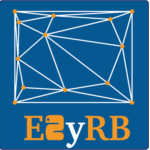
\includegraphics[width=\textwidth]{img/logo_EZyRB_small.png}
	\end{minipage}
	\vspace{-28mm}\hspace{2mm}
	\begin{itemize}
		%\pause
		\item Open source on \texttt{GitHub}
		\item Data driven reduced order modeling framework \\ in python
		\item POD with interpolation (PODI)
	\end{itemize}

	
	
\end{frame}

\begin{frame}{EZyRB}
	\Large{\highlightB{Example Heat Conduction}}
	\normalsize
	
	\begin{minipage}[c]{5.5cm} 
		\begin{equation*}
		\begin{cases}
		- \nabla \cdot (\kappa(x,\mu)\nabla u(x,\mu)) = 0 	& \text{in } \Omega 		\\
		u(x,\mu) = 0 										& \text{on } \Gamma_{top} 	\\
		\kappa(\mu)\nabla u(x,\mu)\cdot \mathbf{n} = 0 		& \text{on } \Gamma_{side} 	\\
		\kappa(\mu)\nabla u(x,\mu)\cdot \mathbf{n} = \mu_1 	& \text{on } \Gamma_{base} 	\\
		\end{cases}
		\end{equation*}
		\begin{align*}
			&\text{find }u(\mu) \in \mathbb{X}:\\
			&a(u(\mu),v;\mu) = f(v;\mu) \quad \forall v \in \mathbb{X}.
		\end{align*}
	\end{minipage}
	\begin{minipage}[c]{5cm} 
		\scalebox{0.75}{
			\tikzset{
	main/.style={black, line width=0.4mm, opacity=1},
	second/.style={gray, opacity=5},
	arrow/.style={-latex, shorten >=1ex, shorten <=1ex, bend angle=45}
}
\begin{tikzpicture}
%% Grid


\node (rect) at (3,3) [draw,main,minimum width=6cm,minimum height=6cm,  fill=blue!30] {};
\draw (3,3) node[circle, main,minimum width=3cm,draw, fill=white] {};
\draw (3,3) node[circle, main,minimum width=3cm,draw, fill=red!60] {};

%\node (rect) at (3,3) [draw,main,minimum width=6cm,minimum height=6cm] {};
%\draw (3,3) node[circle, main,minimum width=3cm,draw, fill=white] {};
%\draw (3,3) node[circle, main,minimum width=3cm,draw] {};


\draw (1,5) node {$\Omega_{2}$};
\draw (2.5 , 3.5) node {$\Omega_{1}$};

\draw (3 , 2) node {$\kappa = \mu_0$};
\draw (2 , 1) node {$\kappa = 1$};

\draw [arrow, main]  ( 3 , 3 ) to ( 4.15 , 4.15 );
\draw (3.75 , 3.35) node {$ r_0 $};

% Rand		
\draw (3 , 6.5) node {$\Gamma_{top}$};
\draw (3 , -0.5) node {$\Gamma_{base}$};
\draw (-0.5 , 3) node {$\Gamma_{side}$};
\draw (6.5 , 3) node {$\Gamma_{side}$};


\end{tikzpicture}
		}
	\end{minipage}
	\begin{align*}
		a(u,v;\mu) = \int_{\Omega} \kappa(x,\mu)\nabla u(x,\mu) \nabla v(x) dx, 
		\qquad
		f(v;\mu) = \mu_1 \int_{\Gamma_{base}} v ~ ds
 	\end{align*}
\end{frame}

\begin{frame}{EZyRB}
	\Large{\highlightB{Snapshots}}
	\normalsize
	
	\begin{align*}
	\Xi_{train}=
	\left\{
	\begin{pmatrix} 0.5 \\ -0.2 \end{pmatrix},
	\begin{pmatrix} 8.6 \\  0.1 \end{pmatrix},
	\begin{pmatrix} 5.3 \\  0.8 \end{pmatrix},
	\begin{pmatrix} 9.4 \\  0.1 \end{pmatrix},
	\begin{pmatrix} 7.3 \\ -0.8 \end{pmatrix},
	\begin{pmatrix} 0.2 \\  0.8 \end{pmatrix},
	\begin{pmatrix} 3.5 \\ -0.5 \end{pmatrix},
	\begin{pmatrix} 0.3 \\  0.6 \end{pmatrix}
	\right\}.
	\end{align*}
	
	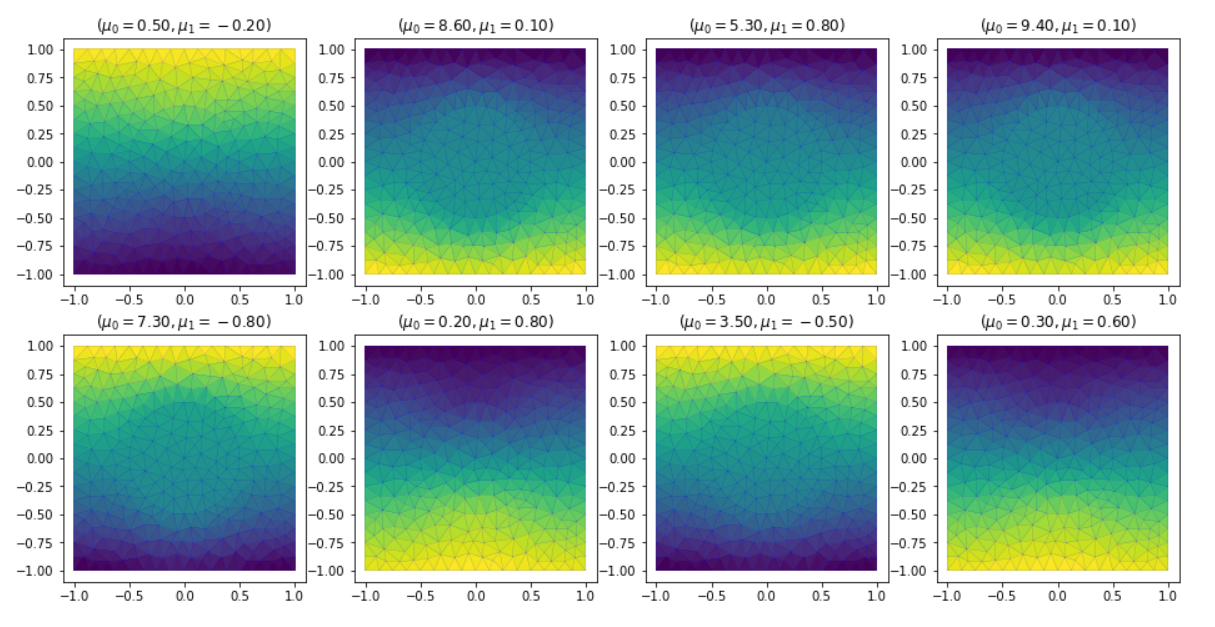
\includegraphics[width=\textwidth]{../images/snapshots}
	
	
\end{frame}

\begin{frame}{EZyRB}
	\Large{\highlightB{Singular values}}
	\normalsize
	
	\centering
	\scalebox{0.75}{
		% This file was created by matlab2tikz.
%
%The latest updates can be retrieved from
%  http://www.mathworks.com/matlabcentral/fileexchange/22022-matlab2tikz-matlab2tikz
%where you can also make suggestions and rate matlab2tikz.
%
\definecolor{mycolor1}{rgb}{0.00000,0.44700,0.74100}%
\definecolor{mycolor2}{rgb}{0.85000,0.32500,0.09800}%
\definecolor{mycolor3}{rgb}{0.92900,0.69400,0.12500}%
%
\begin{tikzpicture}

\begin{axis}[%
width=4.521in,
height=3.566in,
at={(0.758in,0.481in)},
scale only axis,
xmin=0.25,
xmax=8.25,
xlabel style={font=\color{white!15!black}},
xlabel={POD modes},
ymin=0,
ymax=950,
ylabel style={font=\color{white!15!black}},
ylabel={},
axis background/.style={fill=white},
axis x line*=bottom,
axis y line*=left,
legend style={at={(0.97,0.97)}, anchor=north east, legend cell align=left, align=left, draw=white!15!black}
]

\addplot [color=mycolor1, mark=+, mark options={solid, mycolor1, scale=2}]
table[row sep=crcr]{%
	1	874.5893 \\
	2	58.1832  \\
	3	48.2328  \\
	4	45.9105  \\
	5	35.5212  \\
	6	23.8663  \\
	7	20.6150  \\
	8	15.4926  \\
};
%\addlegendentry{Eigen values}

\end{axis}
\end{tikzpicture}%
	}
	
\end{frame}


\begin{frame}{EZyRB}
	\Large{\highlightB{Conclusion}}
	\normalsize

	\begin{itemize}
		\item We presented two algorithms to compute the POD in parallel
		\item EVP perfomes better than SVD due to its limited number of operations
		\item Distributing the snapshot matrix is a bottle neck
		\item We presented hybrid parallel strategy for the POD
	\end{itemize}	

	\vspace{5mm}

	\Large{\highlightB{Outlook}}
	\normalsize
	
	\begin{itemize}
		\item The performance of the computation of the \highlight{correlation matrix} could be improved by using graphics processing units (\highlight{GPU}).
		\
	\end{itemize}
\end{frame}

\begin{frame}{EZyRB}
	\Large{\highlightB{PODmodes}}
	\normalsize
	
	
	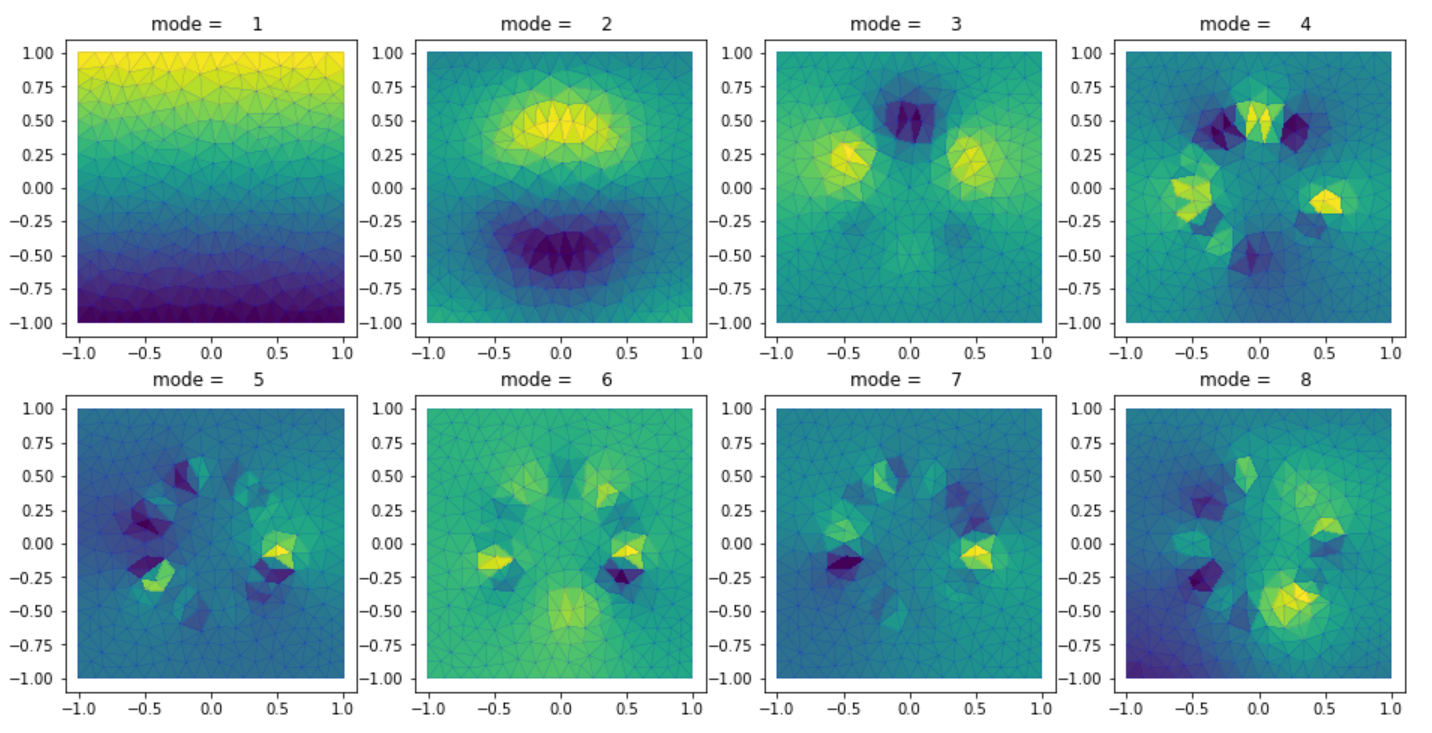
\includegraphics[width=\textwidth]{../images/PODmodes}
	
\end{frame}



